\chapter{Stochastic Optimization}

In this chapter we discuss methods for finding an optima of functions that we are unable to evaluate exactly, but we are able to sample from distribution that is related to such objective function. For example, the objective function might be some characteristics of a random variable. Suppose that pair of random variables $(\mathbf{X}, Y) \in \R^{d+1}$ follows model
\begin{equation*}
	\begin{aligned}
		\E [ Y \vert \X = \x ] & = \mu (\x), \\
		\var [ Y \vert \X = \x ] & = \sigma^2 (\x).
	\end{aligned}
\end{equation*}
where $\mu: \R^d \to \R$ and $\sigma: \R^d \to \Rplus$ are unknown functions. Further suppose that we are able to sample from the conditional distribution $Y \vert \X$.

Denote by $f (y \vert \x)$, $F (y \vert \x)$, and $F^{-1} (\alpha \vert \x)$ the conditional density, cumulative distribution function, and quantile function of $Y \vert \X = \x$.

For the optimization problem
\begin{equation}
	\label{eq:origMax}
	\begin{aligned}
		& \underset{\x}{\max} & & g (\x) \\
		& \st & & \x \in \mathcal{X},
	\end{aligned}
\end{equation}
where $\mathcal{X} \subseteq \R^d$ is given set, we will consider following objective functions
\begin{enumerate}[\itshape i)]
	\item $g (\x) = \mu (\x)$,
	\item $g (\x) = \mu (\x) - \alpha \sigma^2  (\x), \qquad \alpha > 0$,
	\item $g (\x) = F^{-1} (\alpha \vert \x), \qquad (0 < \alpha < 1)$, and
	\item $g (\x) = \E [Y \vert Y \leq F^{-1} (\alpha \vert \x), \X = \x ], \qquad (0 < \alpha < 1)$.
\end{enumerate}

The optimization problem with objective function in \emph{ii} is called Markowitz problem in portfolio theory. The last two objective functions stand for Value at Risk (VaR) and Conditional Value at Risk (CVaR). These optimization problems are well known and the reader can find more about these in any literature about stochastic optimization. We will focus on situations when the functions $\mu$ and $\sigma$ are not known but we are able to generate pairs $(\X, Y)$.

Denote by $\x^{*}$ the optimal point and by $g^{*} = g(\x^{*})$ the optimum of the problem. Note that $\x^{*}$ need not be unique for some problems. In such cases, we will use it to denote whole set of optimal points. The maximization and minimization problems are mutually reversible and, therefore, we will only consider maximization problems in this thesis.

We have already stated, that the distribution of the pair of random variables $(\mathbf{X}, Y)$ is unknown. Also, the function $g$, optimal point $\x^{*}$, and optimum $g^{*}$ are unknown (in sense that we cannot explicitly state it). In this chapter we will propose and study simulation methods for estimating solution to the problem. For that, we simulate random sample $(\X_1, Y_1), ..., (\X_n, Y_n)$ from a population $(\X, Y)$. This data will be used for estimation of the objective function.

The data needs to be generated in way that $Y_1 \vert \X_1, ..., Y_n \vert \X_n$ are mutually independent. Let us not make any assumptions about the distribution of $\X$. Variables $\X_1, ..., \X_n$ need not to be independent or identically distributed.

In following chapters, we briefly introduce two optimization methods for given problem. Both of them are iterative and use the simulated data described above. The first method, a response surface method, seeks for the optimum locally and updates the decision variable based on data generated close to the actual value of the decision variable. On the other hand, the second method, a cross entropy method for optimization, seeks for the optimum globally, uses all information available and selects the values that perform the best.





%%%%%%%%%%%%%%%%%%%%%%%%%%%%%%%%%%%%%%%%%%%%%%%%%%%%%%%%%%%%%%%%%%%%%%%%%%%%%%%%%%%%%%%
%%%%%%%%%%%%%%%%%%%%%%%%%%%%%%%%%%%%%%%%%%%%%%%%%%%%%%%%%%%%%%%%%%%%%%%%%%%%%%%%%%%%%%%
\section{Response Surface Method}
	\label{chap:responseSurface}
	

The idea of the response surface method is to estimate the objective function $g$ and maximize the estimate. Let us denote $\widehat{g}_n$ the estimate of the function $g$ based on random sample of size $n$. Let us consider a bounded set $\mathcal{X}_0 \subseteq \mathcal{X}$ that contains the optimal point, i.e. $\x^{*} \in \mathcal{X}_0$. The set $\mathcal{X}_0$ is our best guess of where the optimal point could be and we are able to estimate the objective function on it. The reason for reduction of the set will be described later. Than we can derive a maximization problem from the initial problem~\eqref{eq:origMax}. The problem can be written in form
\begin{equation}
	\label{eq:derivMax}
	\begin{aligned}
		& \underset{\x}{\max} & & \widehat{g}_n (\x) \\
		& \st & & \x \in \mathcal{X}_0.
	\end{aligned}
\end{equation}
Let us also denote by $\widehat{\x}^{*}_n$ the optimal point and by $ \widehat{g}^{*}_n \equiv \widehat{g}_n (\widehat{\x}^{*}_n)$ the optimum of problem~\eqref{eq:derivMax}. We will call $\widehat{\x}^{*}_n$ and $\widehat{g}^{*}_n$ \emph{estimated optimal point} and \emph{estimated optimum} of problem~\eqref{eq:origMax}. We are also interested in $g (\widehat{\x}^{*}_n)$, which is the value of the objective function at the estimated optimal point. This value is, however, unknown and we try to estimate it.

Obviously, the problem has two main parts that should be solved. First, we need to estimate the objective function $\widehat{g}_n (\x)$. Second, this objective function needs to be maximized. Here we start with the second part. Later, we find out that more than the objective function $g$ needs to be estimated for the purpose of optimization.

We briefly introduce two iterative methods for numerical optimization. That is we take an initial point $\x^{(0)}$. Then we iteratively update $x_k \mapsto x_{k+1}$ until the sequence $x_0, x_1, ...$ reaches selected criterion. Both of the methods are described in \cite{Kroese11}, Appendix C. Then, we generalize these two numerical methods to be applicable in simulated optimization. In the same book, in Chapters 11 and 12, different methods for simulated optimization are described. 

Let us suppose that the derivatives of $g$ exist and are known. Denote by $\nabla_{g} (\x)$ the gradient of $g$ at $\x$. The \emph{gradient descent} method updates the sequence in form
\[
	\x^{(k+1)} = \x^{(k)} + \alpha_k \nabla_{g} (\x^{(k)}),
\]
where $(\alpha_k)_{k=1}^{\infty}$ is sequence of (typically small) step sizes. Intuitively, it is appropriate to take sequence for which
\[
	\alpha_k \to 0 \text{ as } k \to \infty, \qquad \sum_{k=0}^{\infty} \alpha_k = \infty.
\]
Let us further assume that also the second derivatives of $g$ exist and are known and the Hessian, $\nabla^2_{g} (\x)$, is invertible on $\mathcal{X}_0$. The \emph{Newton's method} updates the sequence in form
\[
	\x^{(k+1)} = \x^{(k)} - (\nabla^2_{g} (\x^{(k)}))^{-1} \nabla_{g} (\x^{(k)}).
\]

These methods are applicable only if the derivatives were known. However, alike the function $g$, its derivatives are also unknown. These needs to be estimated as well. Denote by $\widehat{\nabla_g} (\x)$ and $\widehat{\nabla_g^2} (\x)$ the estimated gradient and estimated Hessian of $g$ at point $\x$. Instead of estimating single function, one needs to estimate $d+1$ functions (function $g$ and its derivatives) for gradient method and $(d+1)(d+2)/2$ functions for Newton's method. This indicates that the gradient method becomes more suitable for high-dimensional problems.

With this setup, there are several questions to be answered. In this chapter we try to find answers for these questions.
\begin{itemize}
	
	\item
	How to estimate the objective function $g$ and its derivatives? This, obviously, depends on the type of the function. Different techniques will be used, for example, for mean and for quantile.
	
	\item
	How large should the simulated sample be in order to get close to the actual optimum? For example, in sense of
	\[
		\pr [ g (\widehat{\x}^{*}_n ) \leq g^{*} - \varepsilon ] < \delta
	\]
	for suitable parameters $\varepsilon, \delta > 0$.
	
	\item
	How to construct subset $\mathcal{X}_0$? How to sample variables $\X_1, ..., \X_n$? These two questions are strongly related and need to be answered together.
	
\end{itemize}

Clearly, there are no general answers to those questions that could be applied to every single problem. The reader should be aware that the proposed solutions are reliable to the problems stated in this thesis. On the other hand, it should give an intuition of how to find answer to different problems.

One of the simplest possibilities to estimate the objective function is polynomial regression. The advantages of this approach are that fitting a polynomial is relatively computationally undemanding and polynomial function $\widehat{g}$ is easy to maximize numerically (or even analytically). On the other hand, there are many dependencies for which the polynomial regression fails. See, for example, Figure~\ref{fig:mcycle}.

\begin{figure}[t]
	\centering
	
	\begin{subfigure}[b]{0.45\textwidth}
    \centering
		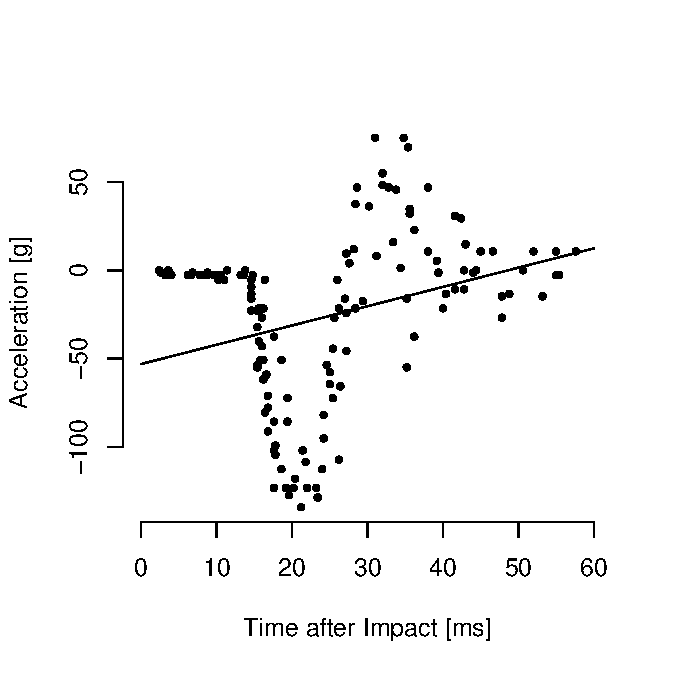
\includegraphics[width=\textwidth]{\FIGDIR/mcycle_p1}
    \caption{Linear regression}
  \end{subfigure}
	\hfill
	\begin{subfigure}[b]{0.45\textwidth}
    \centering
		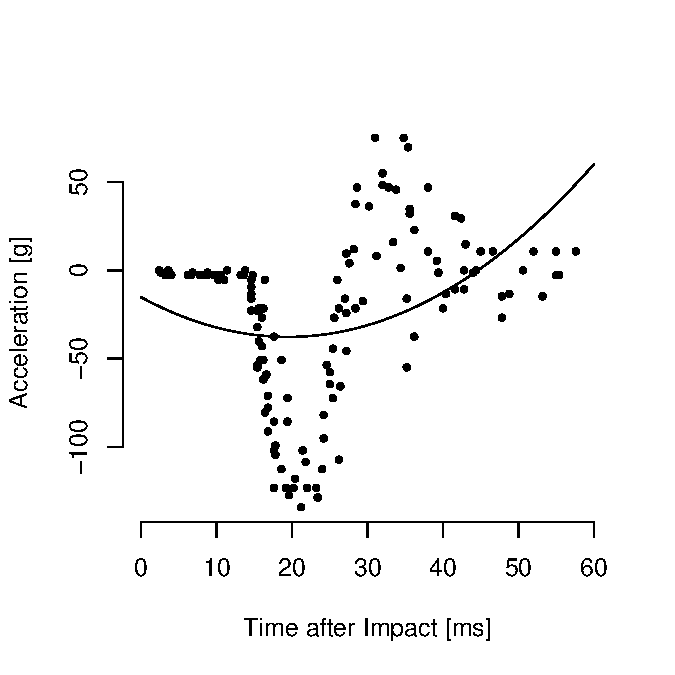
\includegraphics[width=\textwidth]{\FIGDIR/mcycle_p2}
    \caption{Quadratic regression}
  \end{subfigure}

	\begin{subfigure}[b]{0.45\textwidth}
    \centering
		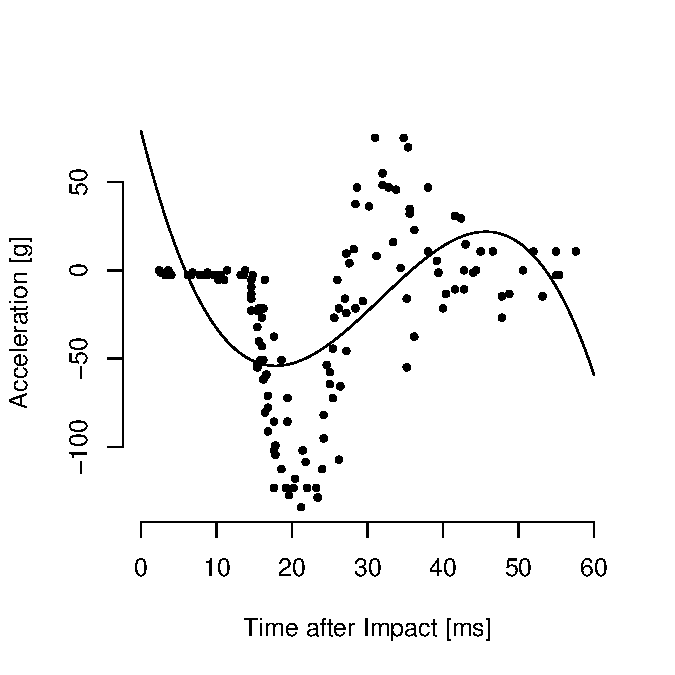
\includegraphics[width=\textwidth]{\FIGDIR/mcycle_p3}
    \caption{Kubic regression}
  \end{subfigure}
	\hfill
	\begin{subfigure}[b]{0.45\textwidth}
    \centering
		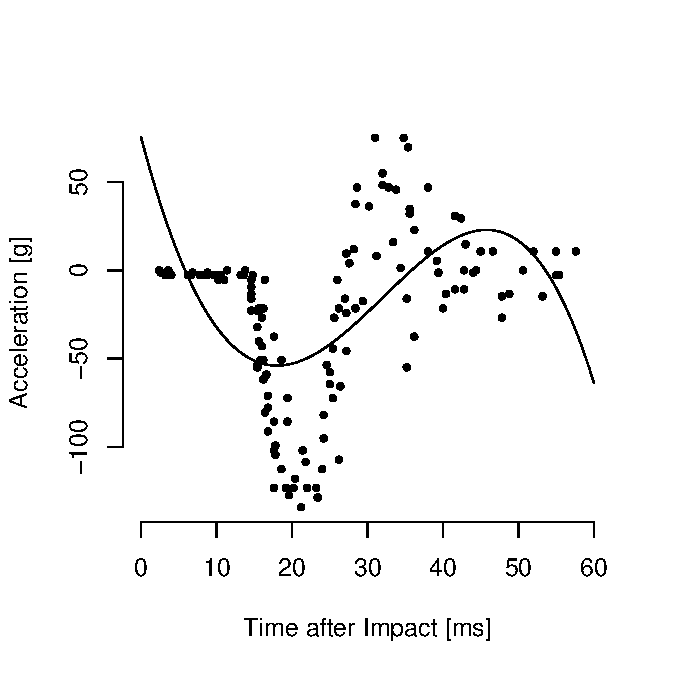
\includegraphics[width=\textwidth]{\FIGDIR/mcycle_p4}
    \caption{Quartic regression}
  \end{subfigure}

	\caption{Polynomial fits to the motorcycle data. The bias of estimates is large even in case of high-order polynomials. The plots are adapted from~\cite{Fan03}.}
	\label{fig:mcycle}
\end{figure}

Another solution is to estimate the objective function locally for each value $\x \in \mathcal{X}$. For that, we assign weights to individual observations based on their distance from $\x$. The further the point is, the lower the weight is. Also, it is possible to assign zero weights to observations from certain distance and exclude these points from estimation. Let us assign the weights to individual observations with a kernel function.

\begin{definition}
	Let $K: \R \to \R$ be a real function satisfying
	\[
		\int_{\R} K(x) dx = 1, \qquad
		\int_{\R} x K(x) dx = 0, \qquad
		0 < \int_{\R} x^2 K(x) dx < \infty
	\]
	Then we call $K$ a \emph{kernel function}.
\end{definition}

\cite{Cleveland79} proposed also other properties that a weight function should have. These are non-negativity, symmetry around zero, monotonicity for all non-negative values, and zero values outside the unit circle. The first three properties are fulfilled for the majority of common kernel functions. The fourth property is reasonable especially for computational purposes, but there are several kernel functions that violate this property. Later, we will see that symmetry of kernel function is unnecessary for our purpose.

Clearly, any density function of a non-degenerate random variable with zero mean and finite variance is a kernel function. Three common examples are the Gaussian kernel
\[
	K(x) = \frac{1}{\sqrt{2 \pi}} \exp \left( - \frac{x^2}{2} \right),
\]
the Epanechnikov kernel
\[
	K(x) = \begin{cases}
		\frac{3}{4} (1-x^2) \qquad & \text{if } \vert x \vert \leq 1 \\
		0 \qquad & \text{else,}
	\end{cases}
\]
and the Tricube kernel
\[
	K(x) = \begin{cases}
		\frac{70}{81} (1 - \left| x \right|^3)^3 \qquad & \text{if } \vert x \vert \leq 1 \\
		0 \qquad & \text{else.}
	\end{cases}
\]
The Tricube kernel was originally proposed by \cite{Cleveland79} and is implemented in R software, package stats, function loess.

Assume that the estimated function is $\mu (\x) = \E [ Y \vert \X = \x ]$. Then the \emph{local polynomial estimator} is in form of
\begin{equation}
	\label{eq:locReg}
	\begin{aligned}
		\widehat{\mu} (\x) = & \widehat{\varphi}_{\x} (\0) \\
		\widehat{\varphi}_{\x} = & \underset{\varphi}{\argmin} & & \sum_{i=1}^n K \left( \frac{ \left\| \X_i - \x \right\| }{h_{\alpha}(\x)} \right) (Y_i - \varphi (\X_i-\x))^2 \\
		& \st & & \varphi \text{ is a polynomial of degree } p.
	\end{aligned}
\end{equation}
Function $\left\| \cdot \right\|$ is the Euclidean norm of a vector. Function $h_{\alpha} (\x)$ is distance between $\x$ and $r$-th closest variable within $\X_1, ..., \X_n$, where $r = \left\lceil \alpha n \right\rceil$. By selecting the kernel function $K$ we control the weights of individual simulations. The span $\alpha$ and the degree $p$ of polynomial $\varphi$ are also of our choice.

We can use the estimated polynomial $\widehat{\varphi}_{\x}$ to estimate also derivatives of mean function by setting
\begin{align*}
	\widehat{\nabla_{\mu}} (\x) &= \nabla_{\widehat{\varphi}_{\x}} (\0), \\
	\widehat{\nabla_{\mu}^2} (\x) &= \nabla_{\widehat{\varphi}_{\x}}^2 (\0).
\end{align*}
For the gradient descent method, we need the local polynomial at least linear ($p \geq 1$). For the Newton's method, we need at least quadratic polynomials ($p \geq 2$).

Let us introduce a method that combines the gradient descent method and the Newton's method. We estimate the second-order derivative of the objective function only as a diagonal matrix. There are two main reasons for not estimating whole Hessian. First, the number of parameters that needs to be estimated is too high and the method is computationally demanding for high-dimensional problems. Second, the Newton's method needs the Hessian (or estimated Hessian) to be invertible. If the matrix is diagonal with non-zero diagonal elements, the inverse always exists. We can define the iterative method as
\begin{equation}
	\label{eq:hybridMethod}
	x^{(k+1)}_i =
		\begin{cases}
			x^{(k)}_i - \displaystyle{\frac {\widehat{\nabla}_{g,i} (\x^{(k)}_i)} {\widehat{\nabla}^2_{g,i,i} (\x^{(k)}_i)}},  & \widehat{\nabla}^2_{g,i,i} (\x^{(k)}_i) < -\frac{1}{\alpha_k} \\
			x^{(k)}_i + \alpha_k \widehat{\nabla}_{g,i} (\x^{(k)}_i), & \text{else,}
		\end{cases}
\end{equation}
where $\widehat{\nabla}_{g,i}$ and $\widehat{\nabla}^2_{g,i,i}$ denote the estimated derivatives of the objective function with respect to $x_i$. The condition on the first line of the definition of the next iteration has two reasons. First, we want to use the second derivatives only if the function is locally estimated as concave down. Second, we want to keep the algorithm stable even around estimated inflexion points where the estimated second derivative is close to zero.

\begin{algorithm}[Response Surface]\
	\label{algo:stochApprox}
	\begin{enumerate}
		\item Set initial value $\x^{(0)}$ and put $k := 0$.
		\item Generate data (multiple independent observations) from distribution $(\X, Y)$, where the predictors $\X$ have the distribution centered at $\x^k$. Join the data with previously generated data (if any).
		\item Fit the local polynomial regression at point $\x^{(k)}$. If the estimated first-order derivatives of $\mu$ are sufficiently close to zero then continue with step 5.
		\item Update $\x^{(k+1)}$ by~(\ref{eq:hybridMethod}) based on estimated derivatives, increase $k := k+1$ and repeat steps 2--4.
		\item Return value $\x^{(k)}$.
	\end{enumerate}
\end{algorithm}

Note that the algorithm does not return the estimated optimum of given problem. The reason for that is that local polynomial regression provides, in general, biased estimate of the estimated function. One can generate multiple observations from distribution $Y \vert \X = \widehat{\x}^{*}$.

Let us illustrate the method on simple example of finding an optimum of exponential of an paraboloid.

\begin{example}
	\label{ex:paraboloidSurface}
	Let $Y = \e^{- \left\| \x \right\|^2} + \varepsilon$, where $\x \in \R^2$ and $\varepsilon \sim N(0,1)$. Suppose that the optimization problem is
	\begin{equation*}
		\begin{aligned}
			& \underset{\x}{\max} & & \mu (\x) \\
			& \st & & \x \in \R^2.
		\end{aligned}
	\end{equation*}
	Clearly, the optimum is $\mu^{*} = 1$ at point $\x = (0,0)^{\top}$. However, we want to estimate the optimum using the Algorithm~\ref{algo:stochApprox}.
	
	We set the initial guess $\x^{(0)} = (1,1)^{\top}$ and at $k$-th iteration we generate 10~000 simulations with distribution of predictors as $\X \sim N_2 (\x^{(k)}, 0.01 \times \mathbb{I}_2)$, where $\mathbb{I}_2$ is $2 \times 2$ unit matrix. The sequence of steps lengths was defined as $\alpha_k = \frac{0.6}{\sqrt[3]{k+1}}$. At $k$-th iteration we used $\frac{0.75}{\sqrt{k+1}} \times 100\%$ nearest observations to fit the polynomial regression with Epanechnikov kernel as weights.
	
	The average distance of the estimated optimum from the actual optimum was 0.074 (confidence interval: 0.046--0.101). The mean number of iterations was 23.3. Some paths of the algorithm and all the estimated optimums are visualized in Figure~\ref{fig:paraboloidSurface}.
	
	\begin{figure}[t]
		\centering
		
			\begin{subfigure}[b]{0.45\textwidth}
				\centering
				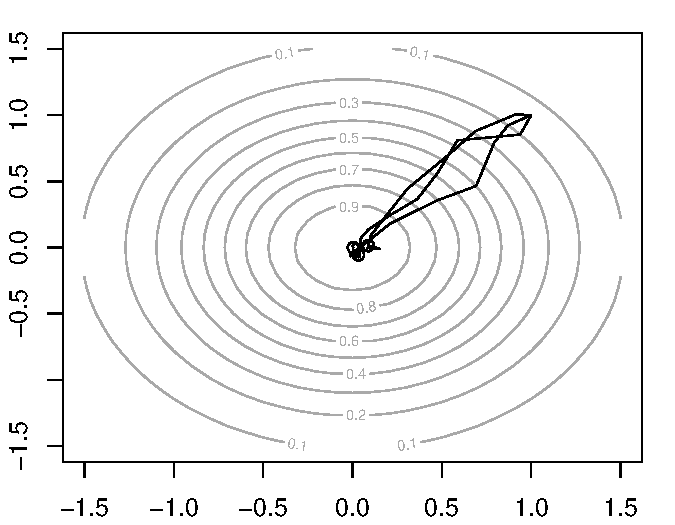
\includegraphics[width=\textwidth]{\FIGDIR/paraboloid_surface_path}
				\caption{Paths of three runs.}
			\end{subfigure}
			\hfill
			\begin{subfigure}[b]{0.45\textwidth}
				\centering
				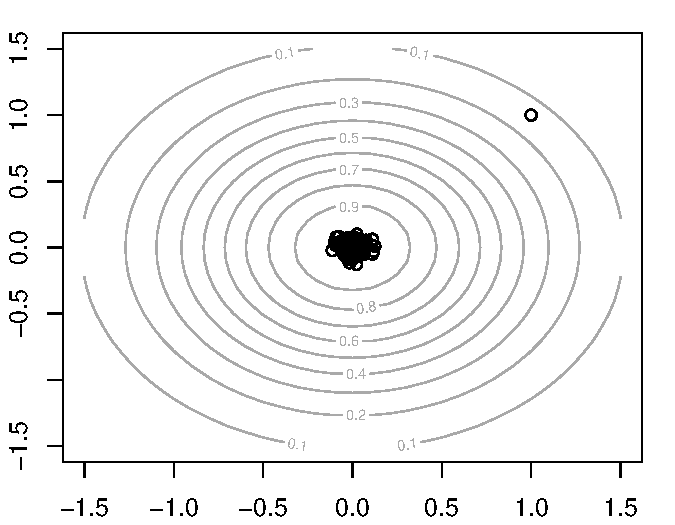
\includegraphics[width=\textwidth]{\FIGDIR/paraboloid_surface_endpoint}
				\caption{End points of 100 runs.}
			\end{subfigure}

		\caption{Visualized results of response surface method from Example~\ref{ex:paraboloidSurface}.}
		\label{fig:paraboloidSurface}
	\end{figure}

	\demo
\end{example}

Until now, we supposed only mean function as the objective function. The method can be generalized for various other functions. One can easily replace the local polynomial regression with any other local model. For example, by using the local quantile regression we can maximize the Value at Risk of random variable $Y \vert \X = \x$. For more local models that could be applied in the response surface method see~\cite{Fan03}.



%%%%%%%%%%%%%%%%%%%%%%%%%%%%%%%%%%%%%%%%%%%%%%%%%%%%%%%%%%%%%%%%%%%%%%%%%%%%%%%%%%%%%%%
%%%%%%%%%%%%%%%%%%%%%%%%%%%%%%%%%%%%%%%%%%%%%%%%%%%%%%%%%%%%%%%%%%%%%%%%%%%%%%%%%%%%%%%
\section{Cross Entropy Method}
	\label{chap:crossEntropy}
	
	Another way to find the optimum of given function with a noise is to use the cross entropy method. This method searches for the optimum by narrowing the set over which the objective function is optimized. In general, this method does not estimate the maximum of the conditional mean as the response surface method does. Also, only a little is known about the convergence of the algorithm.
	
	The algorithm has two main steps. In the first step, the independent values are generated from some distribution and the values that performs the best are selected for the second step. In the second step, the sampling distribution is updated based on the best performances from the first step. It is suitable to use the sampling distributions fixed up to the choice of the distribution parameter and update only the parameter.
	
	Following algorithm is adapted from \cite{Kroese11}.

\begin{algorithm}[Cross Entropy for Noisy Optimization]\
	\label{algo:crossEntropy}
	\begin{enumerate}
		\item Set initial parameter $\bm{\psi}^{(0)}$ and counter $k := 1$.
		\item Generate data (multiple independent observations) of size $n$ from distribution $(\X, Y)$, where the predictors have the distribution $\X \sim f( \;\cdot\; ; \bm{\psi}^{(k-1)})$. Let $\gamma_k$ be the $(1-\varrho)$-quantile of $Y_1, ..., Y_n$.
		\item Estimate the parameter $\bm{\psi}^{(k)}$ from the best performing observations using maximum likelihood
		\[
			\bm{\psi}^{(k)} = \underset{\psi}{\max} \sum_{\X_i \geq \gamma_k} \log ( f ( \X_i; \bm{\psi} ) ).
		\]
		\item If the distribution $f( \;\cdot\; ; \bm{\psi}^{(k)})$ is almost degenerated then continue with step 6, otherwise increase $k := k+1$ and repeat steps 2--4.
		\item Return value $\x$ such that the distribution $f( \;\cdot\; ; \bm{\psi}^{(k)})$ is almost degenerated at point $\x$.
	\end{enumerate}
\end{algorithm}

In the previous algorithm, the stopping criterion is vaguely described as \emph{almost degenerated distribution} $f( \;\cdot\; ; \bm{\psi})$. We use the 1-norm of the variance matrix of the distribution. If the norm is sufficiently close to zero we say that the distribution is almost degenerated.

To compare the algorithm with the response surface method, we use the cross entropy to solve the same problem as we did in previous chapter.

\begin{example}[Continuation of Example~\ref{ex:paraboloidSurface}]
	\label{ex:paraboloidCrossEntropy} 
	We choose to use bivariate normal distribution as the sampling distribution. We set the initial parameters for the distribution as $\mu = (1,1)^{\top}$ and $\sigma^2 = 5 \times \mathbb{I}_2$, where $\mathbb{I}_2$ is $2 \times 2$ unit matrix. The best performances in each iteration are selected using median, i.e. $\varrho = 0.5$.
	
	The average distance of the estimated optimum from the actual optimum was 0.036 (confidence interval: 0.033--0.038). The mean number of iterations was 28.2. Some paths of the algorithm and all the estimated optima are visualized in Figure~\ref{fig:paraboloidCE}.
	
	\begin{figure}[t]
		\centering
		
			\begin{subfigure}[b]{0.45\textwidth}
				\centering
				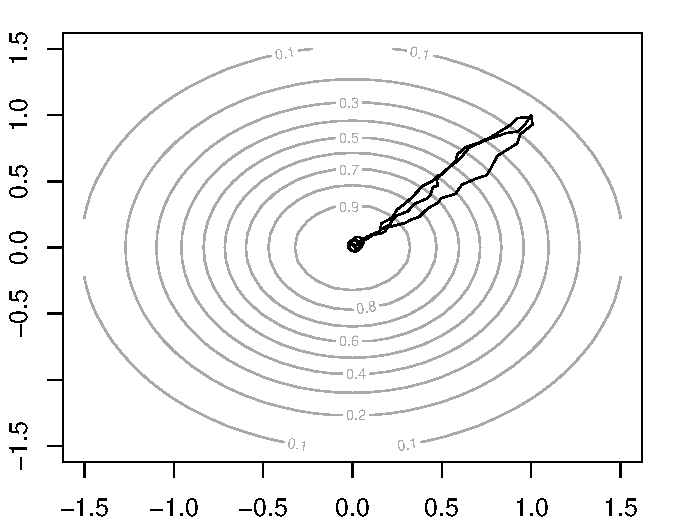
\includegraphics[width=\textwidth]{\FIGDIR/paraboloid_CE_path}
				\caption{Paths of three runs.}
			\end{subfigure}
			\hfill
			\begin{subfigure}[b]{0.45\textwidth}
				\centering
				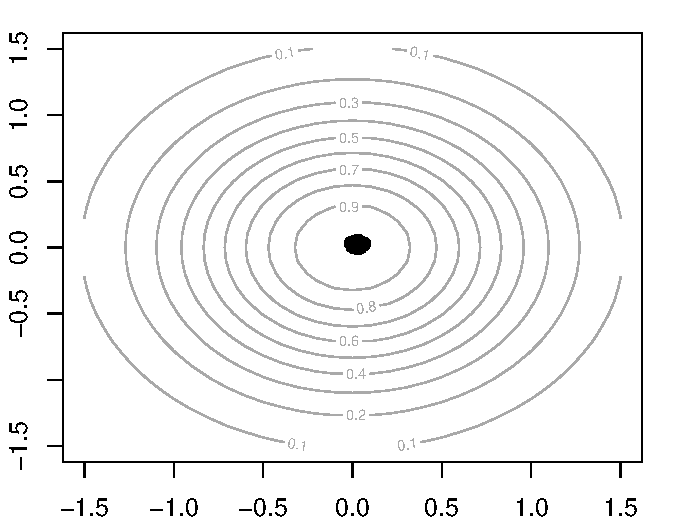
\includegraphics[width=\textwidth]{\FIGDIR/paraboloid_CE_endpoint}
				\caption{End points of 100 runs.}
			\end{subfigure}

		\caption{Visualized results of cross entropy method from Example~\ref{ex:paraboloidCrossEntropy}.}
		\label{fig:paraboloidCE}
	\end{figure}
		
	The cross entropy algorithm provided better results in only a few more iterations. Additionally, this method is computationally less demanding, because we do not need to estimate regression model at each iteration and we do not need to keep all the generated data.

	\demo
\end{example}

Another possibility is to combine both described methods. One could use the cross entropy method to find a solution that will be used as the initial point for the response surface method. By doing this, there are already generated data before the first iteration of the response surface algorithm. Also, the initial point might be closer to the actual solution than the initial guess would be.



%%%%%%%%%%%%%%%%%%%%%%%%%%%%%%%%%%%%%%%%%%%%%%%%%%%%%%%%%%%%%%%%%%%%%%%%%%%%%%%%%%%%%%%
%%%%%%%%%%%%%%%%%%%%%%%%%%%%%%%%%%%%%%%%%%%%%%%%%%%%%%%%%%%%%%%%%%%%%%%%%%%%%%%%%%%%%%%
\section{Multistage Optimization}
	\label{chap:multistage}

Until now, we considered only single-stage problems with one ($d$-dimensional) decision variable. In this chapter, we introduce a method for solving problems with several points in time when the decision has to be done. However, we still consider problems that need to be solved using one of the simulation method. We also need to add one variable to the model to track the history of the realized uncertainty. We considered general objective function $g$ for the simple problems. For the multistage problems we consider only mean function $g = \mu$ for the objective function.

For the $M$-stage stochastic problem we consider following assumptions. Let $\x_1, ..., \x_{M} \in \mathcal{X} \subset \R^d$ be the decision variables. Suppose that the constraints for the decision variable $\x_m$ depends on the very previous decision $\x_{m-1}$ for $m = 2, ..., M$. Denote the largest set that fulfills such constraints by $\mathcal{X} (\x_{m-1})$. Let $\varepsilon_1, ... \varepsilon_M$ be the sequence of random variables that we call the uncertainty of the problem. Suppose the uncertainty depends on the last decision. Then we talk about the \emph{endogenous uncertainty}. Let $\z_0, ..., \z_M \in \S$ be the random variables identifying the state of the decision model. Suppose the number of states is at most countable. The states depend on the very previous state, the last decision and the realization of the uncertainty. One can write $\z_m = \z_m (\z_{m-1}, \x_{m}, \varepsilon_m)$ for $m = 1, ..., M$. Since the state has a random variable as an argument it is random itself as well and it is natural to talk about its distribution. The state $\z_0$ is known (deterministic) prior to the first decision. The dynamics of the model is illustrated in Figure~\ref{fig:dynamics}~(a).

\begin{figure}[t]
	\centering
	
		\begin{subfigure}[b]{\textwidth}
			\centering
			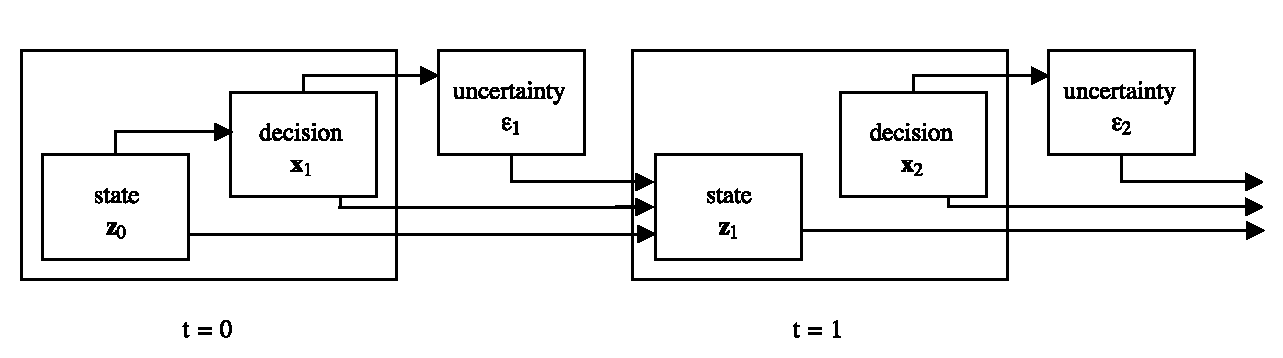
\includegraphics[width=\textwidth]{\FIGDIR/diagramEndogenous}
			\caption{Endogenous uncertainty.}
		\end{subfigure}
		%\vspace*{150px}
		\begin{subfigure}[b]{\textwidth}
			\centering
			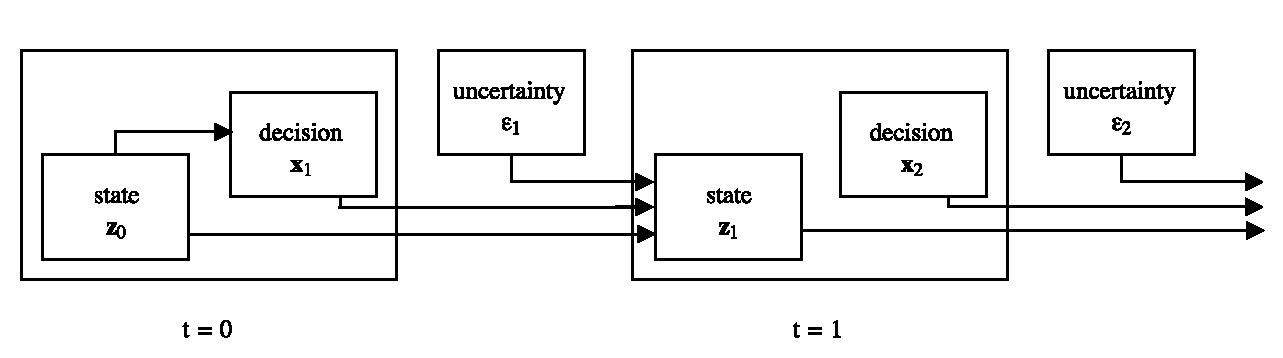
\includegraphics[width=\textwidth]{\FIGDIR/diagramExogenous}
			\caption{Exogenous uncertainty.}
		\end{subfigure}

	\caption{Comparison between the dynamics of the state-space decision model with endogenous and exogenous uncertainty. Adapted from \cite{Pflug14}.}
	\label{fig:dynamics}
\end{figure}

Let the objective random variables be denoted by $Y_m = h (\z_m, \z_{m-1}, \x_{m})$ for $m=1, ..., M$, where $h: \R^{2c+d} \to \R$ is a measurable function. The variable $Y_m$ is usually called a \emph{transition reward}. Denote the expected reward in the $m$-th time interval by $g_{m} (\x_{m}, \z_{m-1}) = \E [Y_m \vert \x_{m}, \z_{m-1}]$. Let the multistage problem be
\begin{equation}
	\label{eq:multistageMax}
	\begin{aligned}
		G_0 = & \underset{\x_1, ..., \x_{M}}{\max} & & \sum_{m=1}^M  g_m (\x_{m}, \z_{m-1})\\
		& \st & & \x_1 \in \mathcal{X}, \\
		&  		& & \x_m \in \mathcal{X} (\x_{m-1}), \qquad m = 2, ..., M.
	\end{aligned}
\end{equation}
Similarly, we can write recursive problems for $m = 1, ..., M-1$
\begin{equation}
	\label{eq:recursiveMax}
	\begin{aligned}
		G_m (\x_{m}, \z_{m}) = & \underset{\x_{m+1}, ..., \x_{M}}{\max} & & \sum_{k=m+1}^M  g_k (\x_{k}, \z_{k-1})\\
		& \st & & \x_k \in \mathcal{X} (\x_{k-1}), \qquad k = m, ..., M.
	\end{aligned}
\end{equation}
Note the state $\z_{m}$ is unknown (depends on unobserved the uncertainty $\varepsilon_{m}$) at time $m$ and, therefore, is random. Since the problem~(\ref{eq:recursiveMax}) depends on $\z_{m}$ it is random as well. \cite{Pflug14} showed that the problem~(\ref{eq:multistageMax}) is equivalent to
\begin{equation}
	\label{eq:reformMax}
	\begin{aligned}
		& \underset{\x_1, ..., \x_{M}}{\max} & & g_1 (\x_{1}, \z_{0}) + \E [G_1 (\x_{1}, \z_{1})] \\
		& \st & & \x_0 \in \mathcal{X}.
	\end{aligned}
\end{equation}

Suppose that we are able to evaluate (generate random variable from such distribution) the function $G_1 (\x_{1}, \z_{1})$. Then we can use some of the method described in Chapters~\ref{chap:responseSurface} and~\ref{chap:crossEntropy} to find the optimum of~(\ref{eq:reformMax}).

Evaluation of $Q_1 (\x_{0}, \z_{1})$ consists of two parts: generating the uncertainty $\varepsilon_1$ and solving the stochastic problem with $M-1$ stages and known initial state $\z_1 (\varepsilon_1)$. If $M=2$ then the problem is easy to solve. For larger problems we need to iterate through the procedure until the problem at the end is single-stage.


